% WOAH 2026 long paper, camera-ready, ACL style, [final] mode.

\documentclass[11pt]{article}
\usepackage[final]{acl}
% For a [review] rebuild, uncomment the next line: lineno's default running
% mode prints numbers in the opposite column at page breaks. [final] does not
% load lineno, so leaving it active here would be an undefined control sequence.
%\AtBeginDocument{\runningpagewiselinenumbers}
\usepackage{times}
% The ACL template's mono family, replacing Courier. Load after times.
\usepackage{inconsolata}
\usepackage{latexsym}
\usepackage{amsmath,amssymb,amsthm}
\usepackage{booktabs}
\usepackage{float}
\usepackage{placeins}
\usepackage{graphicx}
\usepackage{dsfont}
\usepackage{xspace}
\usepackage{enumitem}
\setlist[itemize]{leftmargin=*,topsep=2pt,itemsep=1pt,parsep=0pt,partopsep=0pt}
\setlist[enumerate]{leftmargin=*,topsep=2pt,itemsep=1pt,parsep=0pt,partopsep=0pt}

\newtheorem{proposition}{Proposition}

\newcommand{\dataset}{\textsc{GoldStandard2024}\xspace}
\newcommand{\Fpos}{\ensuremath{F_1^{+}}\xspace}
\newcommand{\CFRh}{\ensuremath{\mathrm{CFR}_{\mathrm{hard}}}\xspace}
\newcommand{\CFRs}{\ensuremath{\mathrm{CFR}_{\mathrm{soft}}}\xspace}
\newcommand{\JS}{\ensuremath{\mathrm{JS}_b}\xspace}
\newcommand{\Indi}{\mathds{1}}
\newcommand{\Loss}{\mathcal{L}}
\newcommand{\bth}{{\boldsymbol{\theta}}}

\title{Counterfactual Robustness and the Calibration Trap in Antisemitism Detection}

\author{
  Giacomo Case, Yasmin Chaqor and Leonardo Cartesegna \\
  EPFL, Lausanne, Switzerland \\
  \texttt{\{giacomo.case, yasmin.chaqor, leonardo.cartesegna\}@epfl.ch}
}

% acl.sty loads hyperref, so configure it once the package exists.
\AtBeginDocument{\hypersetup{
  pdftitle={Counterfactual Robustness and the Calibration Trap in Antisemitism Detection},
  pdfauthor={Giacomo Case, Yasmin Chaqor, Leonardo Cartesegna},
  pdfsubject={Proceedings of the Workshop on Online Abuse and Harms (WOAH) 2026},
  pdfkeywords={hate speech detection, antisemitism, counterfactual robustness,
    calibration, fairness},
}}

\begin{document}
\maketitle

\begin{abstract}
Classifiers for antisemitism detection inherit a shortcut from keyword-sampled training data: predictions flip when a Jewish identity term is rewritten to another religion, even though the gold label is preserved. We audit this fragility jointly along three axes (positive-class performance, calibration, counterfactual stability) and report a previously unquantified tension. While four group-conditional post-hoc calibrators all improve global calibration (ECE), they inflate the soft counterfactual flip rate by $15$--$80\%$. A formal proposition shows intercept-free rescaling cannot change hard flips. \emph{Orbit-constrained calibration} resolves it: it penalises calibrated probability differences on development-set identity-swap pairs, recovering the calibration gain (ECE $-46\%$) with the hard rate unchanged; it is the only calibrator we test that lowers ECE without inflating soft flips. Separately, we attack invariance at training time: CCI (Counterfactual Consistency Invariance) adds a Jensen--Shannon consistency penalty between each tweet and its religiously rewritten counterfactuals. This cuts the hard flip rate by 49--73\% across three encoder backbones and two model families, while preserving or improving \Fpos{} (up to $0.72$). Plain counterfactual augmentation reaches a lower flip rate at $3\times$ the training-set size; raising CCI's multiplier closes that gap at a matched predicted-positive rate. Three prompted 7--8B LLMs cap at \Fpos{} $0.45$, and the two with measured pair sweeps flip an order of magnitude more often. Finally, Integrated Gradients show identity-token attribution nearly unchanged: the gain comes from coupling pair scores, not from suppressing identity salience.
\end{abstract}

\noindent\textbf{Content warning:} this paper contains masked antisemitic slurs and offensive content.

\section{Introduction}
\label{sec:intro}

Antisemitic abuse online causes documented harm to Jewish communities, and platform moderation of it fails in both directions: hateful content survives while legitimate political speech is removed. The boundary is hard. Under the International Holocaust Remembrance Alliance (IHRA) Working Definition~\citep{ihra2016working}, criticism of Israeli policy ``similar to that levelled against any other country'' is not antisemitic, while antisemitism may surface through coded tropes rather than identity terms~\citep{becker2025decoding}.

Supervised detectors make this boundary worse. Corpora collected through Jewish-related keywords inherit identity-token shortcuts: in \dataset{}~\citep{jikeli2024goldstandard}, positive base rates range from $11.4\%$ on \emph{Jews} to $88.3\%$ on \emph{Z*oNazi}. Empirical risk minimisation fits these keyword marginals rather than the IHRA boundary, so predictions flip under religious-identity swaps (\emph{Jew}$\to$\emph{Muslim}) that preserve the label, the operational signature of a model that reads identities instead of content.

Despite a decade of identity-term bias work in hate speech detection, antisemitism detection has drawn relatively little attention at this venue: the one prior WOAH treatment~\citep{ron2023factoring} contributes an annotation framework and an anti-Jewish hate corpus, but does not study detection robustness or the calibration--fairness interaction we audit here. We treat it as a stress test for counterfactual-fairness methods, on a target whose criticism-vs-hate boundary is contested by design. Concretely, we probe the religious-identity axis of that boundary (does renaming the targeted group flip the verdict?); its geopolitical axis (criticism of Israel) motivates the problem but stays outside our swap operator (\S\ref{sec:method}).

\textbf{Contributions.}\footnote{Code, configurations and the pair manifest: \href{https://doi.org/10.5281/zenodo.22699004}{10.5281/zenodo.22699004}. No tweet text is redistributed; see the Ethics Statement.}
\begin{itemize}[leftmargin=1.2em,itemsep=2pt,topsep=2pt]
\item \emph{A calibration--invariance tension, and a post-hoc calibrator that resolves it.} Across four group-conditional calibrators (temperature, Platt, isotonic, HKRR multicalibration~\citep{hebertjohnson2018multicalibration}), every one that lowers Expected Calibration Error (ECE) inflates the soft counterfactual flip rate. A formal proposition shows that intercept-free rescaling cannot move hard flips at the symmetric threshold. We then introduce \emph{orbit-constrained calibration}, which penalises calibrated probability differences on development-set counterfactual swap pairs. This is the one calibrator we test that escapes the trade-off. To our knowledge this is the first quantification of the trade-off, and the first post-hoc fix, for abuse detection. \item \emph{A three-axis audit of antisemitism detection} (positive-class $F_1$, \Fpos; ECE; counterfactual flip rates) with Holm-corrected significance over six seeds. This includes a null result: group error-rate parity (false-negative equality difference, FNED) neither improves nor degrades. \item \emph{CCI (Counterfactual Consistency Invariance)}, a training-time Jensen--Shannon consistency loss over religiously symmetric identity swaps. Where Counterfactual Logit Pairing (CLP)~\citep{garg2019counterfactual} and its extension to hate speech~\citep{davani2021improving} penalise an unbounded $L_p$ logit gap, our JS penalty is a bounded surrogate that Pinsker's inequality ties to the hard flip rate. Its gradient vanishes on already-consistent pairs, rather than pressuring confident pairs whose probabilities already agree. CCI cuts the hard counterfactual flip rate (\CFRh) by 49\%/58\%/73\% across DeBERTa-v3-base/large and RoBERTa-large at \Fpos{} up to $0.72$, transferring across tokeniser and model families. Counterfactual augmentation reaches a lower flip rate at $3\times$ the training-set size; CCI attains that regime as a drop-in loss, closes the remaining gap when its multiplier is raised (App.~\ref{app:lambda}), and flips less than augmentation at a quarter of the labels (App.~\ref{app:semisup}).
\end{itemize}

\section{Related Work}
\label{sec:related}

\textbf{Identity-term shortcuts and counterfactual pairing.} \citet{dixon2018measuring} introduced FPED/FNED and documented identity-term shortcuts as the dominant weakness of hate-speech corpora. Keyword-stratified sampling of the kind that built \dataset{}~\citep{jikeli2023antisemitic} acts before training and does not constrain the learned function on individual pairs. \citet{garg2019counterfactual} penalise the $L_p$ logit difference between a sentence and its identity swap; \citet{davani2021improving} extend this to hate speech. Both operate in unbounded logit space and have been validated within a single backbone family.

\textbf{Counterfactual evaluation and training.} Counterfactual invariance in abuse detection has mostly been treated as an evaluation problem. HateCheck~\citep{rottger2021hatecheck} instantiates templated functional tests across seven protected groups, Jewish people not among them, which supports comparison across groups rather than paired swap invariance, and \citet{fryer2022flexible} generate flexible counterfactuals for fairness probing; both diagnose models but leave training untouched. Counterfactual fairness~\citep{kusner2017counterfactual} formalises invariance over a causal graph, rarely available for noisy social-media text; our operator instead operationalises the causal intervention via identity-term rewriting. Our flip rate is the thresholded, paired analogue of perturbation sensitivity analysis~\citep{prabhakaran2019perturbation}. Closest to our approach is counterfactual data augmentation (CDA) ~\citep{lu2020gender,zmigrod2019counterfactual,kaushik2020learning}, which trains on rewritten pairs without an explicit consistency term. CCI extends this paradigm by coupling the rewrites with a Jensen--Shannon penalty. Recent work in abuse detection probes adjacent axes without coupling them to calibration: counterfactual token fairness for Dutch detection~\citep{bauer2025fairness}, identity-swapped functional tests across Singapore languages~\citep{ng2024sghatecheck}, and concept-sufficiency diagnosis without a corresponding mitigation~\citep{nejadgholi2023concept}.

\textbf{Calibration and multicalibration.} Temperature scaling~\citep{guo2017calibration} is monotone and cannot move decisions across the symmetric threshold (\S\ref{sec:method}). Multicalibration~\citep{hebertjohnson2018multicalibration} guarantees subgroup calibration but, as we quantify, breaks individual invariance. The inherent conflict between calibration and fairness is well established: \citet{pleiss2017fairness} show that calibration and equalised odds are incompatible outside degenerate cases, while calibration remains compatible with a single error-rate constraint such as equal false-negative rates. That result concerns a different axis from ours (calibration vs.\ counterfactual invariance under identity swaps), and the tension we document is not an impossibility: an orbit-constrained map avoids it. \citet{fillies2025taxonomy} organise mitigation methods by operation principle and annotate each with its pipeline stage. Our orbit calibrator and CCI loss sit in their post-processing and in-training cells; what we add is the measured interaction between the two. Recent audits of dataset robustness and representation~\citep{antypas2023robust,korre2023harmful,tonneau2024languages} likewise treat calibration and counterfactual stability separately; we measure their interaction.

\section{Method}
\label{sec:method}

\textbf{Setup.} Let $(X, Y, S) \sim \mathcal{D}$, where $X$ is a tweet, $Y \in \{0,1\}$ its IHRA label, and $S$ its dataset collection-keyword stratum; FNED is reported over the four values of $S$; ECE is global unless stated. Calibration instead uses $G = g(X) \in \{\textsc{Jews, Israel, K*kes, Z*oNazi, none}\}$, the group our identity inventory infers from the text itself. The two need not agree, and a rewritten input is regrouped from its own text. A classifier $f_\bth$ produces logits $(z_0(X), z_1(X))$; we use the decision logit $z_\bth(X) = z_1(X) - z_0(X)$, posterior $p_\bth(X) = \sigma(z_\bth(X))$, and hard prediction $\hat Y_\bth(X) = \Indi\{p_\bth(X) \ge 1/2\}$.

\textbf{Counterfactual operator.} An operator $\Psi$ generates a set of up to five rewrites per tweet, replacing a Jewish religious-ethnic token (\emph{jew, jewish, hebrew, judaism}), while preserving case, with one of \{\emph{muslim, christian, hindu, buddhist, atheist}\}. A pair $(X,X')$ is admissible only if it survives three filters. First, no slur may be involved (\emph{k*ke}, \emph{z*onazi}, \emph{chr*stkiller}), since slur-bearing text changes meaning under substitution. Second, the mention must be religious-ethnic rather than a purely geopolitical proxy (\emph{Israel}, \emph{Zionist} with no religious anchor). Third, implicit conspiracy-only references (\emph{globalist}, \emph{Rothschild}, \emph{Soros}) are excluded because they encode the target without naming it. The operator targets the religious-ethnic component of the shortcut: geopolitical-only swaps are excluded because their labels need not survive the rewrite under the IHRA boundary. The filter removes the religious-ethnic anchor, not every residual reference: $18\%$ of admissible pairs retain a geopolitical proxy the rewrite does not move, so label preservation on the remainder is an assumption rather than a guarantee. Under that label-preservation assumption, $\Psi$ induces a pair distribution $\mathcal{Q}$; its test realisation $\mathcal{P}$ has $2{,}117$ pairs generated from $611$ of the $1{,}060$ test tweets. We call $\{X\}\cup\Psi(X)$ the \emph{swap orbit} of $X$.

\begin{figure*}[t]
\centering
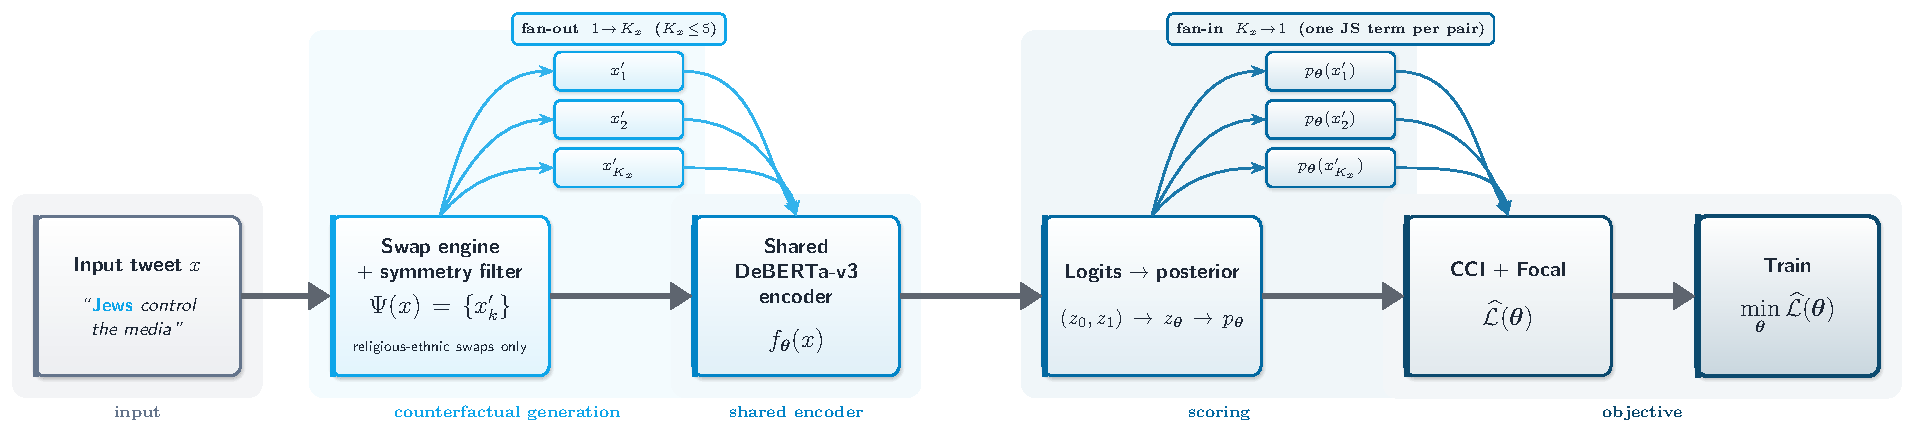
\includegraphics[width=\textwidth]{../figures/cci_v2_pipeline_blue.pdf}
\caption{CCI pipeline. A shared encoder scores a tweet $x$ and its religiously rewritten counterfactuals $x'_k$; the training loss couples their predictions with a Jensen--Shannon penalty.}
\label{fig:pipeline}
\end{figure*}

\textbf{Objective.} Intuitively, we train the standard classifier while requiring that admissible identity rewrites do not change its decisions (Figure~\ref{fig:pipeline}). Formally,
\begin{equation}\label{eq:constrained}
\min_{\bth}\ \mathbb{E}_\mathcal{D}\!\left[\ell_{\mathrm{focal}}(f_\bth(X),Y)\right]\ \ \text{s.t.}\ \ \CFRh(\bth) \le \varepsilon,
\end{equation}
where $\ell_{\mathrm{focal}}$ is the focal loss~\citep{lin2017focal} (the corpus is $4.79{:}1$ imbalanced) and $\CFRh(\bth) = \mathbb{E}_\mathcal{Q}\,\Indi\{\hat Y_\bth(X) \ne \hat Y_\bth(X')\}$ is the hard flip rate, non-differentiable since $\hat Y_\bth$ thresholds a continuous score. The companion soft metric is $\CFRs^{L_1}(\bth) = \mathbb{E}_\mathcal{Q}\,|p_\bth(X){-}p_\bth(X')|$.

\textbf{Smooth surrogate.} Pinsker's inequality applied to each KL summand of the binary Jensen--Shannon divergence gives $\tfrac{1}{2}|p-p'|^2 \le \JS(p,p')$, so \JS{} upper-bounds pairwise disagreement outside a vanishing margin of the threshold. Relaxing \eqref{eq:constrained} with a fixed multiplier $\lambda{=}1$, held at one value across every backbone and cell rather than tuned per condition (App.~\ref{app:lambda}), yields the training loss
\begin{equation*}
\begin{aligned}
\widehat{\Loss}_B(\bth) = {}& \frac{1}{|B|}\sum_{i\in B}\ell_{\mathrm{focal}}(f_\bth(X_i),Y_i) \\
&+ \frac{\lambda}{N_B}\sum_{i\in B}\sum_{k=1}^{K_i}\JS\bigl(p_\bth(X_i),p_\bth(X'_{ik})\bigr).
\end{aligned}
\end{equation*}
Here $B$ is a minibatch of training tweets, $K_i \le 5$ (zero for tweets with no admissible rewrite) is the number of admissible counterfactuals for $X_i$, and $N_B = \sum_{i\in B}K_i$; the consistency term is zero when $N_B{=}0$. Valid pairs, not tweets, carry equal weight. Operationally, the \JS{} term is a smooth, bounded stand-in for the flip rate: its gradient vanishes on pairs the model already treats consistently and pulls disagreeing pairs toward their Bernoulli mean. An $L_1$ divergence and a learned temperature head are ablated in App.~\ref{app:extended}.

\begin{proposition}[Sign-preservation of temperature scaling]\label{prop:ts}
For any $T>0$, $\Indi\{\sigma(z/T)\ge 1/2\}=\Indi\{z\ge 0\}$; hence hard predictions at the symmetric threshold are pointwise $T$-invariant and $\CFRh^T(\bth)\equiv\CFRh(\bth)$.
\end{proposition}

\noindent Proposition~\ref{prop:ts} rules out every intercept-free monotone rescaling of the decision logit at the symmetric threshold; a post-hoc remedy must move the decision boundary itself (an affine or per-cell correction). We show below that the natural per-cell candidate, multicalibration, buys ECE at the cost of soft-flip inflation, so a post-hoc remedy must constrain the map itself (\S\ref{sec:validation}). Training details are in Appendix~\ref{app:training}.

\section{Validation}
\label{sec:validation}

\textbf{Data and protocol.} \dataset{}~\citep{jikeli2024goldstandard} (CC BY 4.0): $11{,}311$ English tweets keyword-sampled around \{\emph{Jews, Israel, K*kes, Z*oNazi}\}, annotated under the IHRA definition by the dataset's curators. We use a stratified $80/10/10$ split ($8{,}479/1{,}060/1{,}060$; $187$ test positives) of the $10{,}599$ tweets remaining after removing duplicate texts, which the corpus contains and which would otherwise leak across splits, and report \Fpos, $15$-bin ECE, \CFRh{} and $\CFRs^{L_1}$ over $\mathcal{P}$, and the false-negative equality difference (FNED)~\citep{dixon2018measuring}.
Adapting paired bootstrap resampling~\citep{dror2018hitchhikers} to seed-level test-set statistics, each contrast resamples the six training seeds with replacement ($10^4$ resamples; the unit is the seed-level test-set scalar, not individual examples or pairs), with Holm--Bonferroni correction applied separately within two pre-specified families at family-wise $\alpha{=}0.05$: 54 pivot-vs-comparator tests and 6 within-architecture transfer tests. Because the $10^4$ resamples floor the bootstrap $p$-value at $10^{-4}$ when all six seeds agree in direction, we also report an exact two-sided sign test over seeds (minimum $p = 2\cdot 2^{-6} \approx 0.031$, uncorrected) as a direction-consistency check. All cells aggregate six seeds ($42$--$47$).

\begin{table*}[t]
\centering
\small
\setlength{\tabcolsep}{3pt}
\begin{tabular}{lccccc}
\toprule
Method & $\Fpos\uparrow$ & ECE$\downarrow$ & $\CFRh\downarrow$ & $\CFRs^{L_1}\downarrow$ & FNED$\downarrow$ \\
\midrule
C (DeBERTa-base)                   & $.660{\pm}.019$ & $.077{\pm}.034$ & $.036{\pm}.008$ & $.032{\pm}.006$ & $.797{\pm}.159$ \\
\;\;+ TempScaling                  & $.660{\pm}.019$ & $.045{\pm}.014$ & $.036{\pm}.008$ & $.033{\pm}.009$ & $.797{\pm}.159$ \\
\;\;+ Multicalibration             & $.646{\pm}.022$ & $\mathbf{.035}{\pm}.005$ & $.033{\pm}.006$ & $.057{\pm}.013$ & $.957{\pm}.064$ \\
Davani CLP ($\lambda{=}0.5$)       & $.672{\pm}.015$ & $.094{\pm}.033$ & $.040{\pm}.005$ & $.036{\pm}.005$ & $.786{\pm}.036$ \\
CDA (augment-only)                 & $.662{\pm}.012$ & $.070{\pm}.028$ & $\mathbf{.012}{\pm}.004$ & $\mathbf{.013}{\pm}.001$ & $.775{\pm}.105$ \\
\textbf{CCI} (DeBERTa-base)     & $.677{\pm}.008$ & $.098{\pm}.053$ & $.018{\pm}.003$ & $.014{\pm}.002$ & $.793{\pm}.180$ \\
\midrule
C (DeBERTa-large)                  & $.704{\pm}.020$ & $.097{\pm}.053$ & $.042{\pm}.003$ & $.037{\pm}.009$ & $\mathbf{.612}{\pm}.051$ \\
\textbf{CCI} (DeBERTa-large)    & $\mathbf{.721}{\pm}.012$ & $.096{\pm}.057$ & $.017{\pm}.009$ & $.016{\pm}.003$ & $.655{\pm}.056$ \\
C (RoBERTa-large)                  & $.689{\pm}.016$ & $.068{\pm}.044$ & $.047{\pm}.002$ & $.048{\pm}.001$ & $.708{\pm}.064$ \\
\textbf{CCI} (RoBERTa-large)    & $.694{\pm}.005$ & $.077{\pm}.052$ & $.013{\pm}.006$ & $\mathbf{.013}{\pm}.002$ & $.759{\pm}.115$ \\
\midrule
LLM Llama-3.1-8B, Guided-CoT       & .450 & --   & --               & --   & --   \\
LLM Mistral-7B, best prompt        & .417 & --   & $.168^{\dagger}$ & --   & --   \\
LLM Qwen-2.5-7B, best prompt       & .373 & --   & $.238$           & --   & --   \\
\bottomrule
\end{tabular}
\caption{Test metrics on \dataset{} ($n{=}1{,}060$); $\CFRh$ and $\CFRs^{L_1}$ over $\mathcal{P}$ ($|\mathcal{P}|{=}2{,}117$). Encoder cells are mean$\pm$std over six seeds; Model~C is the focal-loss baseline with keyword masking: during training only, and with probability $0.3$, the eight collection keywords (\emph{jews, jewish, israel, israeli, zionist, zionazi, kike, kikes}) are replaced by the tokeniser's mask token. It is named Model~C throughout. Guided-CoT follows \citet{patel2025evaluating}. LLM \Fpos{} is over parseable responses from each model's best prompt, whereas the reported LLM \CFRh{} values are zero-shot ($^{\dagger}$Mistral \CFRh{} over its $69\%$ parsed pairs; $[.116,.427]$ full-denominator); the LLM dashes need probabilities the models do not expose. Coverage in App.~\ref{app:llm}. Bold = per-column winner.}
\label{tab:main}
\end{table*}

\textbf{Main result.} Table~\ref{tab:main} reports a \CFRh{} reduction of 49\% on DeBERTa-v3-base, 58\% on DeBERTa-v3-large and 73\% on RoBERTa-large versus the same-architecture Model~C row, masked where CCI is not (App.~\ref{app:factorial}). Holm-corrected paired bootstrap rejects equality on both CFR metrics in every contrast against the four base-architecture comparators (Model~C, its temperature-scaled variant, multicalibration and Davani CLP) and in both large-backbone cells ($p_{\mathrm{boot}}{=}10^{-4}$ for these comparisons). An exact seed-level sign test agrees in every cell ($p{=}0.031$).

\textbf{Error-rate parity.} At fixed backbone the FNED difference is within seed noise in every same-architecture contrast after Holm correction (Model~C, its temperature-scaled variant, Davani $\lambda{=}0.5$, and post-hoc multicalibration); the largest gap, a nominal improvement over multicalibration whose per-cell correction widens group error-rate disparity, does not survive correction (uncorrected $p{=}.03$). \Fpos{} is preserved or improved at every cell.

\textbf{Against augmentation.} Counterfactual augmentation (CDA, the same admissible swaps as hard-labelled rows) reaches a lower hard flip rate (\CFRh{} $.012$ at \Fpos{} $.662$): what cuts flips is exposure to the swap set with the pair coupled, as data or as a bounded consistency penalty; Davani CLP's unbounded logit penalty does not. CCI reaches that regime as a drop-in loss without the 3$\times$ training-set expansion CDA requires. That margin closes when the multiplier is raised: at $\lambda{=}5$ CCI reaches \CFRh{} $.009$ at \Fpos{} $.666$ and a predicted-positive rate of $.147$ against CDA's $.154$ (paired \CFRh{} $-.003$, $p{=}.11$; \Fpos{} $+.004$, $p{=}.59$; App.~\ref{app:lambda}). A keyword-masking factorial (App.~\ref{app:factorial}) shows that the $\lambda{=}1$ margin is not a masking artefact and that CCI's reduction survives matched masking: the C-to-CCI \CFRh{} reduction is $50\%$ with masking on and $54\%$ with it off, CDA keeps a $33$ to $35\%$ edge in both columns, and masking itself moves \CFRh{} by $\le.004$ while lowering \Fpos{} (most for CCI, whose swaps operate on the identity tokens masking removes). 

\textbf{Portability.} The largest reduction crosses tokeniser families (SentencePiece vs.\ BPE) and model families. CCI generates its rewrites in text space and applies the penalty to predicted probabilities, so the same procedure runs unchanged on either backbone; the observed reductions demonstrate that portability rather than invariance to tokenisation or to logit scaling, which the Jensen--Shannon penalty does not have.

\textbf{Mechanism.} Integrated Gradients~\citep{sundararajan2017axiomatic} show the median fraction of attribution mass on identity tokens is nearly unchanged ($0.046 \to 0.044$; paired Wilcoxon over $500$ test examples, Holm-corrected $p<10^{-2}$, $d_z{=}0.11$), so the gain does not come from suppressing identity-token salience. The \JS{} term instead couples each pair's scores toward their Bernoulli mean, visible directly as the soft flip rate falling from $.032$ to $.014$ (Table~\ref{tab:main}).

\begin{table}[t]
\centering\small
\resizebox{\columnwidth}{!}{%
\begin{tabular}{lccc}
\toprule
Calibrator & ECE$\downarrow$ & $\CFRs^{L_1}$ infl. & $\CFRh$ \\
\midrule
(uncalibrated)          & $.077$ & --              & $.0358$ \\
Per-group temperature   & $.044$ & $+47\%$         & $.0358$ \\
Per-group Platt         & $.030$ & $+15\%$         & $.0347$ \\
Per-group isotonic      & $.030$ & $+48\%$         & $.0334$ \\
Multicalibration (patching) & $.035$ & $+80\%$         & $.0325$ \\
\textbf{Orbit (ours)}   & $.041$ & $\mathbf{-0\%}$ & $\mathbf{.0358}$ \\
\bottomrule
\end{tabular}}
\caption{Post-hoc calibration of Model~C (DeBERTa-v3-base, six seeds), fitted on dev and evaluated over $\mathcal{P}$. Every unconstrained group-conditional calibrator improves ECE but inflates the soft counterfactual flip rate, and the intercept-bearing ones also perturb \CFRh; only the orbit-constrained temperature avoids both.}
\label{tab:calib}
\end{table}

\textbf{The calibration--invariance tension.} Group-conditional post-hoc calibration improves global ECE but pulls counterfactual pairs apart: a tweet (group $g$) and its swap (group $g'$) pass through different per-group corrections, so their probabilities diverge even when their hard predictions agree. Table~\ref{tab:calib} quantifies this on Model~C across four calibrators fitted on dev. All four cut ECE (from $.077$ to $.030$--$.044$) but inflate $\CFRs^{L_1}$ by $15$--$80\%$; the intercept-bearing maps (Platt, isotonic, multicalibration) additionally perturb \CFRh, while intercept-free per-group temperature leaves it bit-exact (Proposition~\ref{prop:ts}) yet still inflates the soft rate by $47\%$. Calibration and counterfactual invariance are in tension for all four standard calibrators. Multicalibration, the one that most directly targets subgroups, implemented as a full-sweep variant of HKRR patching that corrects every violating group-bin cell per pass rather than the single worst, leaves worst-group ECE over the four keyword groups unchanged ($.221$, equal to the uncalibrated base).

\textbf{Orbit-constrained calibration restores the frontier.} The tension is not intrinsic to calibration; it is a property of correcting each group independently. We add an orbit penalty to per-group temperature: fit $\{T_g\}$ on dev to minimise NLL plus $\beta$ times the mean absolute calibrated probability difference over dev swap pairs. This penalises pair-score disagreement without constraining the group temperatures to be equal. Being intercept-free it preserves \CFRh{} bit-exactly for any $\beta$. $\beta$ is selected on dev; at $\beta{=}0$ the penalty is absent, though that member is not identical to the separate per-group temperature baseline, whose optimisation bounds and small-group handling differ. At inference it applies $T_{g(x)}$ by the input's own group, needing no test-time swaps. It cuts ECE by $46\%$ ($.077\to.041$, below unconstrained per-group temperature's $.044$) with zero mean soft-flip inflation (Table~\ref{tab:calib}): the only calibrator we test that lowers ECE without trading away counterfactual invariance. CCI itself is a consistency loss, not a calibrator (its ECE matches or trails its baseline); the two are complementary, training-time invariance plus orbit-aware post-hoc calibration.

\textbf{LLM and out-of-distribution audit.} The three $\le 8$B instruction-tuned models cap at \Fpos{} of $0.450$, $23$--$27$ points below the CCI cells, and the two with measured pair sweeps flip an order of magnitude more often (zero-shot $\CFRh{=}.238$ Qwen at full coverage, $.168$ Mistral over parseable pairs, versus $.013$--$.018$ for CCI): scale and instruction-tuning alone do not confer counterfactual stability at this size. A 70B model scores higher on this corpus~\citep{patel2025evaluating}, where counterfactual stability is not measured. On the Jewish-target subsets of HateXplain~\citep{mathew2021hatexplain} and ToxiGen~\citep{hartvigsen2022toxigen}, baseline and CCI rank comparably (PR-AUC differences within $[-0.007,+0.021]$). The apparent fixed-cutoff gap is a prevalence-shift artefact (mean oracle thresholds for both fall in $[0.06,0.18]$), not a ranking deficit.

\section{Conclusion}
\label{sec:conclusion}

On a contested, under-studied target, naive group-conditional calibration improves calibration only by breaking counterfactual invariance. An orbit-constrained map recovers the calibration gain without that cost. The CCI consistency loss cuts hard flips by $49\%$ to $73\%$ across three backbones at equal or higher \Fpos, as a drop-in term without the $3\times$ training-set expansion augmentation requires; it closes augmentation's remaining flip-rate margin when its multiplier is raised, and flips less than augmentation at a quarter of the labels. Counterfactual robustness and calibration need not conflict, provided the post-hoc map respects the swap orbits. One null result bounds the scope: group error-rate parity (FNED) is neither improved nor degraded.

\section*{Limitations}

The swap vocabulary covers explicit identity terms only; coded antisemitism (\emph{Rothschild}, \emph{globalist}) is tracked but not swapped, and the three admissibility filters are heuristic. The operator also rewrites one occurrence of an identity term per pair, so $713$ pairs keep a residual anchor to the source group; restricting to the rest moves the reported \CFRh{} reduction by at most $4.1$ points, below what a size-matched placebo null resolves at $80\%$ power (App.~\ref{app:validity}). Label preservation itself is not measured here, but if rewrites broke labels at any real rate, a loss that pulls each tweet toward its rewrites would pull \Fpos{} down; instead \Fpos{} rises in all three cells ($.660{\to}.677$, $.704{\to}.721$, $.689{\to}.694$) and its seed spread falls ($.019{\to}.008$, $.020{\to}.012$, $.016{\to}.005$), which is evidence against wholesale breakage rather than a measurement of its rate. All training data and every headline number come from a single English Twitter corpus under one annotation scheme, and the out-of-domain check covers two Jewish-target subsets only; the IHRA definition is contested, and alternatives such as the Jerusalem Declaration~\citep{jd2021jerusalem} draw the Israel-criticism boundary differently, so our labels, and what counts as a ``preserved'' label under a swap, inherit a normative choice. CCI does not improve group error-rate parity (FNED within seed noise) or calibration (ECE degrades or remains on par with the baseline quality). The LLM cells are single-run point estimates evaluated solely on parseable responses; their \CFRh{} is measured zero-shot for two of the three models (Qwen at full coverage, Mistral over the $69\%$ of pairs both sides parse), with the Llama pair sweep left to future work. Counterfactual augmentation (CDA) reaches a lower \CFRh{} than the published \JS{} configuration at $\lambda{=}1$ and full supervision (Table~\ref{tab:main}; the $L_1$ variant flips less still, at a cost in \Fpos{} and ECE, App.~\ref{app:extended}), so a consistency penalty is not the only route to robustness there; raising the multiplier to $\lambda{=}5$ matches CDA's rate at a matched predicted-positive rate (App.~\ref{app:lambda}), without the 3$\times$ training-set expansion CDA requires.

\section*{Ethics Statement}

\textbf{Dual use.} A detector of antisemitism can be repurposed to suppress legitimate political speech; predictions that flip when a religious group is renamed represent one mechanism by which moderation penalises benign mentions of a protected identity, and reducing these flips is our primary goal. We recommend deployment as a triage tool with human review for borderline scores, not autonomous action. The swap operator generates no abusive content and ships with the code; we publish no tweet text and no trained checkpoint, so that care falls to whoever trains and deploys one.

\textbf{Annotation framework.} Our labels follow the IHRA Working Definition because it is the framework of \dataset; the methodological contribution is framework-independent (the loss enforces invariance with respect to whichever labels annotators provide), and practitioners adopting a different framework inherit that framework's boundary judgments. We take no position in the definitional debate and disclose the dependency.

\textbf{Data and content.} Our use of \dataset{}~\citep{jikeli2024goldstandard} is a secondary analysis of a public CC~BY~4.0 release through its own distribution channel: the tweets were gathered without explicit author consent, usernames are masked to \texttt{@USER} and never modelled, the released splits carry tweet identifiers without the author column, and no additional ethics-board review was required. The corpus contains slurs, Holocaust-related content, conspiracy theories, and dehumanising language; we reproduce offensive terms only where scientifically necessary, mask slurs with asterisks, and flag content with a warning. Full provenance, annotation protocol, compute and the artefact release are documented in App.~\ref{app:data}.

\bibliography{woah2026}

\appendix

\section{Data statement}
\label{app:data}

\textbf{Corpus.} \dataset{}~\citep{jikeli2024goldstandard} contains $11{,}311$ English tweets posted between January 2019 and April 2023, curated at Indiana University by random keyword sampling (\emph{Jews}, \emph{Israel}, and the slurs \emph{Z*oNazi}, \emph{K*kes}) from a $10\%$ public-tweet archive~\citep{jikeli2023antisemitic}. The release contains tweet IDs, usernames, and full text, and includes slurs and Holocaust-related content.

\textbf{Annotation.} Each tweet was labelled by two trained annotators who viewed it in live context and applied the IHRA definition. Annotators had prior academic exposure to antisemitism and spanned different religions and genders. Pre-adjudication agreement was Cohen's $\kappa{=}0.66$, measured on the predecessor corpus; disagreements were discussed and unresolved tweets removed~\citep{jikeli2023antisemitic}. Counterspeech that quotes antisemitism is deliberately labelled non-antisemitic, which reduces but does not remove the risk that trained models penalise benign mentions of Jewish identity.

\textbf{Models and compute.} The backbones are DeBERTa-v3-base (184M parameters), DeBERTa-v3-large (435M), and RoBERTa-large (355M). Each training run used a single NVIDIA A100 GPU; sweeps dispatched independent runs concurrently across a shared cluster pool.

\textbf{Implementation.} Models, tokenisers and generation use HuggingFace \texttt{transformers} ($\ge$4.36) on PyTorch ($\ge$2.1); the encoder checkpoints are \texttt{microsoft/deberta-v3-base}, \texttt{microsoft/deberta-v3-large} and \texttt{roberta-large}. The prompted models are \texttt{meta-llama/Llama-3.1-8B-Instruct}, \texttt{mistralai/Mistral-7B-Instruct-v0.3} and \texttt{Qwen/Qwen2.5-7B-Instruct}, loaded in 4-bit via \texttt{bitsandbytes} and decoded greedily. Classification metrics use \texttt{scikit-learn} ($\ge$1.3), the paired bootstrap and sign tests use \texttt{scipy} ($\ge$1.11), and Integrated Gradients uses \texttt{captum} ($\ge$0.7).


\textbf{Release.} We release code, not data: the code, the configurations, the per-seed rollups behind the trained-model tables, a per-split index of tweet ids, and a manifest of the $2{,}117$ pairs with each substitution. No tweet text is redistributed; the corpus is fetched from its own archive and the code rebuilds the splits and the pairs exactly.

\FloatBarrier
\section{Training details}
\label{app:training}
AdamW, learning rate $2{\times}10^{-5}$ (base) / $1{\times}10^{-5}$ (large), weight decay $0.01$ (zero on biases and LayerNorm), $10\%$ linear warm-up, effective batch $16$, gradient clipping at $1$, sequence length $128$, focal $\gamma{=}2$, $\alpha{=}0.75$, fp32, patience-3 early stopping on dev macro-$F_1$, six seeds per cell. The swap operator draws three of the five alternative groups per identity occurrence under a fixed seed, caps rewrites at five per tweet, and substitutes the number- and form-matched surface form (\emph{judaism} to \emph{islam}, \emph{jews} to \emph{muslims}).

\FloatBarrier
\section{LLM evaluation details}
\label{app:llm}
Every prompt of every model, with the share of responses the rule-based parser could map to a label. All three prompting conditions follow \citet{patel2025evaluating}, who introduced them for this task and this corpus. Table~\ref{tab:main} quotes the best prompt per model.

\begin{table}[t]
\centering
\small
\resizebox{\columnwidth}{!}{%
\begin{tabular}{l l c c}
\toprule
Model & Prompt & \Fpos & Valid (\%) \\
\midrule
Llama-3.1-8B-Instruct    & zero-shot  & 0.441          & 99.5  \\
                         & few-shot   & 0.443          & 99.4  \\
                         & Guided CoT & \textbf{0.450} & 83.9  \\
\addlinespace
Mistral-7B-Instruct-v0.3 & zero-shot  & 0.296          & 100.0 \\
                         & few-shot   & \textbf{0.417} & 61.4  \\
                         & Guided CoT & 0.240          & 10.3  \\
\addlinespace
Qwen2.5-7B-Instruct      & zero-shot  & 0.335          & 100.0 \\
                         & few-shot   & \textbf{0.373} & 100.0 \\
                         & Guided CoT & 0.298          & 49.5  \\
\bottomrule
\end{tabular}}
\caption{Prompted-LLM results on the $1{,}060$-tweet test set (greedy decoding); bold marks the best prompt per model. \Fpos{} is over parseable responses; \emph{Valid} is the fraction the rule-based parser mapped to a label. Low-validity cells (e.g.\ Mistral CoT, $10.3\%$) score a non-random subset and are not directly comparable.}
\label{tab:llm-appendix}
\end{table}

\FloatBarrier
\section{Extended results}
\label{app:extended}
The cells behind the Method's choices: Davani CLP at the other multipliers, the divergence and temperature-head ablation that settles on \JS{} with fixed $T$, the per-seed calibration spread behind the ECE caveat in the Limitations, and the per-seed check of Proposition~\ref{prop:ts}.

\begin{table}[htbp]
\centering
\setlength{\tabcolsep}{4pt}
\resizebox{\columnwidth}{!}{%
\begin{tabular}{@{}lcccc@{}}
\toprule
Method & \Fpos & ECE & $\CFRh$ & $\CFRs^{L_1}$ \\
\midrule
Davani $\lambda{=}1.0$            & $.660{\pm}.017$ & $.127{\pm}.047$ & $.034{\pm}.011$ & $.029{\pm}.010$ \\
Davani $\lambda{=}2.0$            & $.667{\pm}.019$ & $.177{\pm}.035$ & $.042{\pm}.009$ & $.026{\pm}.006$ \\
Davani $\lambda{=}1.0$ (no filt.) & $.661{\pm}.025$ & $.162{\pm}.055$ & $.041{\pm}.010$ & $.028{\pm}.004$ \\
\bottomrule
\end{tabular}}
\caption{Davani CLP comparators (DeBERTa-v3-base), six seeds. ``No filt.'' disables the swap-symmetry filter, which raises \CFRh{} from $.034$ to $.041$, so the filter removes spurious swaps at no cost in stability; none of these rows reaches CCI's $.018$ (Table~\ref{tab:main}).}
\label{tab:app_davani}
\end{table}

\begin{table}[htbp]
\centering
\setlength{\tabcolsep}{4pt}
\resizebox{\columnwidth}{!}{%
\begin{tabular}{@{}llcccc@{}}
\toprule
$T_g$ & Div. & \Fpos & ECE & $\CFRh$ & $\CFRs^{L_1}$ \\
\midrule
fixed   & $L_1$ & $.651{\pm}.012$ & $.200{\pm}.019$ & $.007{\pm}.002$ & $.003{\pm}.001$ \\
fixed   & JS    & $.677{\pm}.008$ & $.098{\pm}.053$ & $.018{\pm}.003$ & $.014{\pm}.002$ \\
learned & $L_1$ & $.647{\pm}.010$ & $.186{\pm}.012$ & $.008{\pm}.002$ & $.004{\pm}.000$ \\
learned & JS    & $.662{\pm}.015$ & $.083{\pm}.048$ & $.015{\pm}.008$ & $.013{\pm}.003$ \\
\bottomrule
\end{tabular}}
\caption{CCI ablation (DeBERTa-v3-base): temperature head (fixed vs.\ learned) $\times$ divergence ($L_1$ vs.\ JS), six seeds. $L_1$ cuts $\CFRh$ below even CDA's $.012$ but costs \Fpos{} and ECE; JS is the better trade-off and is the published configuration. Fixed and learned $T$ tie on $\CFRh$ ($p{=}0.25$), so we pivot on fixed-$T$ (row~2).}
\label{tab:app_ablation}
\end{table}

\begin{table}[htbp]
\centering
\small
\resizebox{\columnwidth}{!}{%
\begin{tabular}{@{}lcccccc@{}}
\toprule
Seed & 42 & 43 & 44 & 45 & 46 & 47 \\
\midrule
Model~C ECE & .063 & .054 & \textbf{.129} & \textbf{.109} & .067 & .040 \\
Model~C recall & .647 & .551 & .722 & .636 & .572 & .626 \\
Model~C $F_1$ epoch & 7 & 5 & 3 & 3 & 5 & 4 \\
\addlinespace
CCI ECE & .049 & \textbf{.174} & .078 & \textbf{.149} & .046 & .092 \\
CCI recall & .631 & .733 & .668 & .631 & .610 & .583 \\
\bottomrule
\end{tabular}}
\caption{Per-seed 15-bin ECE and recall for Model~C and CCI (DeBERTa-v3-base); each method's two largest ECE values are bold. Both methods show substantial calibration variation across seeds, and each one's worst-calibrated seed is also its highest-recall seed. Checkpoints were selected by development macro-$F_1$. Six seeds cannot establish bimodality or attribute the spread to the stopping rule.}
\label{tab:app_bimodal}
\end{table}

\begin{table}[htbp]
\centering
\small
\begin{tabular}{@{}lccc@{}}
\toprule
Seed & Fitted $T$ & $\CFRh$ (raw) & $\CFRh$ (TS) \\
\midrule
42 & 1.400 & .0321 & .0321 \\
43 & 1.244 & .0293 & .0293 \\
44 & 0.602 & .0444 & .0444 \\
45 & 0.566 & .0463 & .0463 \\
46 & 1.388 & .0255 & .0255 \\
47 & 0.985 & .0373 & .0373 \\
\bottomrule
\end{tabular}
\caption{Empirical face of Proposition~\ref{prop:ts}: post-hoc temperature scaling (with $T$ fitted on dev, range $0.57$--$1.40$) preserves $\CFRh$ bit-exactly on all six Model~C seeds, since monotone rescaling cannot move any score across the symmetric threshold.}
\label{tab:app_ts}
\end{table}

\FloatBarrier
\section{Keyword-masking factorial}
\label{app:factorial}
Here masking is crossed with the three training methods, to separate CCI's effect from the masking Model~C applies.

\begin{table}[t]
\centering\small
\begin{tabular}{llcc}
\toprule
Metric & Method & mask off & mask on \\
\midrule
$\CFRh$ & focal & $.040$ & $.036$ \\
        & CDA   & $.012$ & $.012$ \\
        & CCI   & $.018$ & $.018$ \\
\addlinespace
\Fpos   & focal & $.667$ & $.660$ \\
        & CDA   & $.673$ & $.662$ \\
        & CCI   & $.677$ & $.647$ \\
\bottomrule
\end{tabular}
\caption{Keyword-masking factorial (DeBERTa-v3-base, six seeds, test split). CCI's \CFRh{} reduction over Model~C survives matched masking ($50\%$ with masking on, $54\%$ off); CDA holds the lowest \CFRh{} in both columns, so its margin at $\lambda{=}1$ is not a masking artefact. Masking itself moves \CFRh{} by at most $.004$ and lowers \Fpos, most for CCI, since it removes the identity tokens the swaps act on. Table~\ref{tab:main} publishes C and CDA with masking on and CCI with it off.}
\label{tab:factorial}
\end{table}


\FloatBarrier
\section{Validity of the counterfactual manifest}
\label{app:validity}

\textbf{Placebo slices.} The operator rewrites one occurrence of an identity term per pair, so $713$ of the $|\mathcal{P}|{=}2{,}117$ pairs keep a residual anchor to the source group. For a slice of $k$ pairs we recompute the \CFRh{} reduction and compare it against $2{,}000$ random slices of the same size, rejecting two-sided when $|s-\bar s_0|$ exceeds the $95$th percentile of $|s_0-\bar s_0|$. \textsc{no-jewish} ($k{=}1{,}404$) retains no Jewish identity term and \textsc{no-anchor} ($k{=}1{,}137$) also drops geopolitical and coded terms; \emph{shorter} ($k{=}1{,}416$, at or below the $66.5$th percentile of length) is a size-matched sham, defined by a criterion unrelated to the defect. MDE$_{80}$ is the smallest location shift of the reference distribution reaching $80\%$ rejection: it measures sensitivity under that assumption, and is not an upper bound on an undetected effect.

\begin{table}[t]
\centering
\footnotesize
\setlength{\tabcolsep}{3.5pt}
\begin{tabular}{llrrc}
\toprule
Backbone & Slice & shift & MDE$_{80}$ & det. \\
\midrule
DeBERTa-base  & \textsc{no-jewish} & $-2.6$  & $7.7$  & no \\
              & \textsc{no-anchor} & $+0.6$  & $10.2$ & no \\
              & \emph{shorter}     & $+10.1$ & $7.5$  & \textbf{yes} \\
\addlinespace
DeBERTa-large & \textsc{no-jewish} & $+4.1$  & $6.7$  & no \\
              & \textsc{no-anchor} & $+2.9$  & $8.8$  & no \\
              & \emph{shorter}     & $-1.0$  & $6.6$  & no \\
\addlinespace
RoBERTa-large & \textsc{no-jewish} & $-0.2$  & $5.0$  & no \\
              & \textsc{no-anchor} & $-0.1$  & $6.6$  & no \\
              & \emph{shorter}     & $-3.5$  & $5.1$  & \textbf{yes} \\
\bottomrule
\end{tabular}
\caption{Swap-operator validity. ``shift'' is the slice reduction minus the
size-matched placebo mean, in points of relative \CFRh{} reduction; MDE$_{80}$ is
the smallest shift the placebo null resolves at $80\%$ power; ``det.'' marks
slices the null rejects. Substantive slices are small-caps, the sham slice
italic. Six seeds per cell, $2{,}000$ placebo replicates.}
\label{tab:validity}
\end{table}

\textbf{Reading.} No substantive slice is distinguishable from random slices of its own size, with $|$shift$|$ at most $4.1$ points against a sensitivity of $5.0$ to $10.2$; unrestricted, the protocol recovers $48.8\%$ against the $49\%$ of Table~\ref{tab:main}. On DeBERTa-v3-base and RoBERTa-large the sham slice is rejected at the same $k$, so the test does resolve shifts of that size there; DeBERTa-v3-large has no such control. The residual anchor therefore leaves no detectable trace at this sensitivity; this is a sensitivity statement, not an equivalence bound.

\FloatBarrier
\section{Label efficiency: CCI against augmentation}
\label{app:semisup}

\textbf{Design.} At labelled fraction $f$ all three methods receive the same
labelled subset; only CCI additionally enforces its consistency term on the
unlabelled remainder, which augmentation cannot use because it needs a label to
copy onto each rewritten row. Six seeds per cell, eighteen at $f{=}0.25$.
Fraction $1.0$ is the main run of Table~\ref{tab:main}, and the sweep reproduces
it (CDA \CFRh{} $.0117$ at \Fpos{} $.662$), which serves as the self-check.

\begin{table}[t]
\centering
\footnotesize
\setlength{\tabcolsep}{4pt}
\resizebox{\columnwidth}{!}{%
\begin{tabular}{rrrrrc}
\toprule
$f$ & $n$ & $\Delta$\CFRh{} & $p_{\mathrm{boot}}$ & sign & Holm \\
\midrule
$0.10$ & $6$  & $-.0106$ & $.0001$ & $6/6$   & rejects \\
$0.25$ & $18$ & $-.0046$ & $.0066$ & $15/18$ & rejects \\
$0.50$ & $6$  & $-.0017$ & $.3008$ & $4/6$   & no \\
$1.00$ & $6$  & $+.0067$ & $.0002$ & $1/6$   & --- \\
\bottomrule
\end{tabular}}
\caption{CCI minus CDA on \CFRh{}, paired over seeds; negative means CCI flips
less. Holm at family-wise $\alpha{=}0.05$ over the sub-$1.0$ fractions, which are
the pre-registered family; $f{=}1.0$ is the published cell and sits outside it.
$p_{\mathrm{boot}}$ cannot fall below the resampling floor of $10^{-4}$, which the
$f{=}0.10$ cell reaches.}
\label{tab:semisup}
\end{table}

\textbf{Reading.} At $f{=}0.25$ CCI cuts \CFRh{} $33\%$ below CDA, with the
paired bootstrap and the sign test agreeing, which is the standard the cells of
Table~\ref{tab:main} meet. At $f{=}0.5$ the difference is small (a standardised effect of $0.42$) and
six seeds do not resolve it; its size implies roughly an order of magnitude more
would be needed. At $f{=}0.1$ CCI's \Fpos{} is $6.7$ points lower, so that cell
is not \Fpos-matched and its larger gap is not interpretable as invariance.

\textbf{Prevalence check.} A model predicting positive less often has fewer predictions available to flip, and at $f{=}0.25$ CCI's \Fpos{} is $.0095$ below CDA's. Regressing the per-seed $\Delta$\CFRh{} on the per-seed $\Delta$\Fpos{} leaves an intercept of $-.0043$ at zero $\Delta$\Fpos{} (uncorrected bootstrap $p{=}.010$, $95\%$ interval $[-.0079,-.0011]$), so the gap does not reduce to the \Fpos{} difference. The direct test, a comparison at matched predicted-positive rates, is the one App.~\ref{app:lambda} applies at full supervision; this cell has the regression only.

\FloatBarrier
\section{Consistency multiplier}
\label{app:lambda}

\textbf{Design.} The multiplier is held at $\lambda{=}1$ throughout the paper:
one value across three backbones, six seeds and every cell of
Table~\ref{tab:main}, rather than a value tuned per condition. This appendix
reports what the multiplier controls. Three further arms at
$\lambda\in\{0.5,2,5\}$ on DeBERTa-v3-base are identical to the published
configuration in every other respect (masking off, six seeds each, the same stopping
rule); $\lambda{=}1$ is the published run itself.

\begin{table}[t]
\centering
\small
\begin{tabular}{lccc}
\toprule
Arm & \Fpos{} & \CFRh{} & pos.\ rate \\
\midrule
$\lambda{=}0.5$ & $.657{\pm}.008$ & $.0207{\pm}.0061$ & $.177$ \\
$\lambda{=}1$   & $.677{\pm}.008$ & $.0183{\pm}.0028$ & $.159$ \\
$\lambda{=}2$   & $.662{\pm}.011$ & $.0144{\pm}.0052$ & $.155$ \\
$\lambda{=}5$   & $.666{\pm}.014$ & $.0089{\pm}.0034$ & $.147$ \\
\midrule
CDA             & $.662$          & $.0117$            & $.154$ \\
\bottomrule
\end{tabular}
\caption{CCI at four multipliers against CDA: DeBERTa-v3-base, test split,
mean${\pm}$std over six seeds per arm; masking off for CCI and on for CDA, as in
Table~\ref{tab:main}. pos.\ rate is the predicted-positive rate on the $1{,}060$
test tweets, listed because a flip rate lowered by predicting fewer positives
would be a move along the operating curve rather than added invariance.}
\label{tab:lambda}
\end{table}

\textbf{Reading.} In Table~\ref{tab:lambda}, \CFRh{} falls monotonically in $\lambda$, from $.0207$ to
$.0089$, while \Fpos{} moves by $.020$ across the whole range. At $\lambda{=}5$
CCI reaches CDA's flip rate: paired over seeds the difference is $-.0028$ in
\CFRh{} (bootstrap $p{=}.11$) and $+.0040$ in \Fpos{} ($p{=}.59$), neither
resolvable at six seeds, and the predicted-positive rates are $.147$ against
$.154$, so the arms are close to matched rather than separated by a shift in
prevalence. The \CFRh{} margin CDA holds at $\lambda{=}1$
(Table~\ref{tab:semisup}, $f{=}1.0$ row, $+.0067$) is a setting we can move, and
moving it closes the margin with \Fpos{} and predicted-positive rate matched to
CDA's ($.666$ against $.662$; $.147$ against $.154$).

We report this as an ablation and do not re-select $\lambda$ on it:
Table~\ref{tab:main} is the $\lambda{=}1$ model throughout, and $\lambda$ was
fixed before any of these arms were trained.


\end{document}
